\documentclass{article}

\usepackage{graphicx}
\usepackage{amsmath}
\usepackage{graphicx}
\graphicspath{{images/}} 

\title{APG4011F Assignment 3}
\date{07/05/2015}
\author{Jason David Russell - RSSJAS005}

\begin{document}

\maketitle
\pagenumbering{gobble}

\newpage
\tableofcontents

\pagenumbering{arabic}

\newpage
\section{Introduction}
The purpose of this assignment is to gain an understading into the principles of image restituion and bundle adjustment.
A python program will be used to demonstrate and simulate how image restituion and bundle adjusment is performed.
The main tasks of this assignment involve creating appropriate ficticouos data so that an image ray intersection, resection
and multiple bundle adjustment can be performed. Thereafter, the actual intersection, resection and bundle adjustment will 
be carried out and results will be compared to the original ficotuous data.


\section{Background}
Image restitution and bundle adjustment has many applications in various fields such as computer vision and photogrammtery. 
The objective of image restituion is to reconstruct image rays and camera attitude in space, as they existed during the moment of photogrophy. 
This means that a single image ray will pass through a perspective center, image point, and homologous object point, and so
in order to reconstruct an image ray, various parameters need to be taken into consideration:
Perspective center cooridantes, camera tilt/attitude, camera focal length/principle distance, image point coordiante (in the 
image coordiante system), and correspsond object point coordiante.
The process of reconstrcuting iamge rays and camera characteristics can be broken down into two main parts, interior and exterior orientation.
Exterior orientation involves paramters concering the camera, while inerior orientation involves paramters of actual image rays.

\newpage

\subsection{Interior Orientaion}
Interioer or Inner orientaiobn is described as the reconstruction of the geomerty of th bundle of imagin rays as they exitsted at the time 
of photogrpay. It is defined by: the calibrated principle distance of the camera, the postion of the principle poing in the image plane, 
and the gemometric distortion characteristics of the lens system.
In this assignement, ficticous image and object points will be created such that an intersection, resection and full bundle adjustment 
can be carried out. 

\begin{figure}[h!]
\centering
\caption{Interior Orientaion dipiction.}
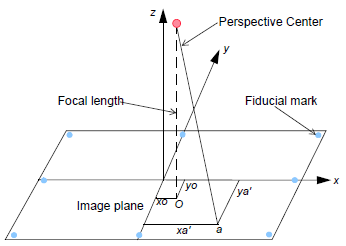
\includegraphics{interior_diagram}
\end{figure}

\begin{figure}[h!]
\centering
\caption{Interior orientaion equations.}
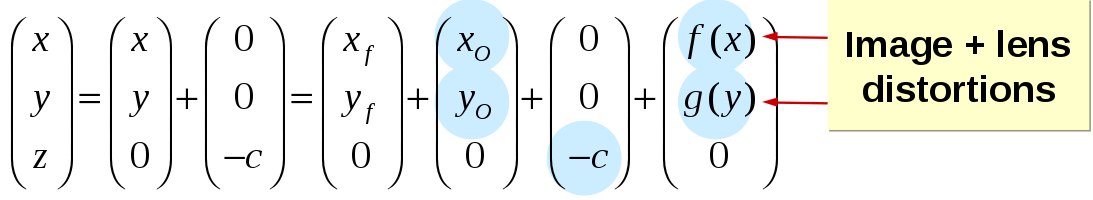
\includegraphics[scale=0.3]{interior_equations}
\end{figure}

\newpage

\subsection{Exterior Orientation}
Exterour or Outer orirenataion is descibed as the reconstruction of the poiition and attitide of the camera as it existed at the time of
photogrpahy and is defined by: the posituion of the projection cener, and the rotaion anges for each 3D axis.

\begin{figure}[h!]
\centering
\caption{Exterior Orientaion dipiction.}
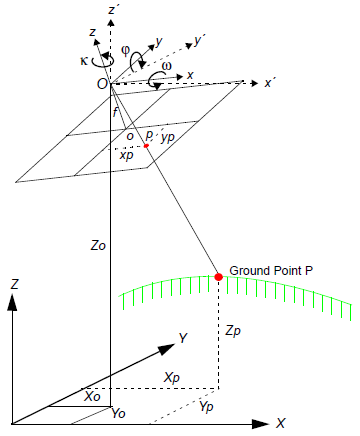
\includegraphics{exterior_diagram}
\end{figure}

\newpage

\subsection{Collinearity Condition}
In order to relate these two systems, the collinearity condition is used and it states that assuming no unmodelled image and lens
distortions, the projection center, object point and correspding image point should lie on a straight line.

\begin{figure}[h!]
\centering
\caption{Collinearity Condition Equations.}
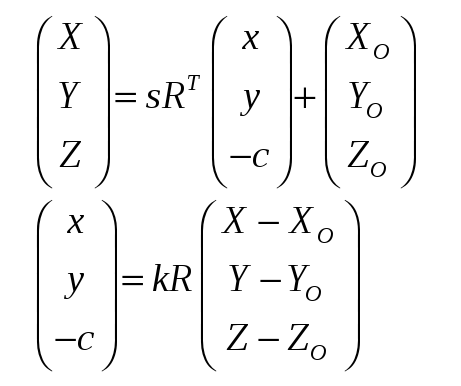
\includegraphics[scale=0.3]{collinearity_equations}
\end{figure}

Bundle adjustment can be defined as the simultaneous refining of 3D coordiantes describing a scene geometery as well 
as the parameters of the realtive motion and optical characteristcs of the cameras used to accuire images, 
accodng to an optially reiterion involving the correspsoding image projections of all points.


\section{Problem Statement}
There are three main questions which will be addressed in this assignment. They are listed below:

\subsection{Intersection}
Given a set of object points which have homolougous points in two seperate images, with each image having unique exterior 
orientation paramters, set up a least squares adjustment using the collieanarity equations to redetermine the object points 
from each pair of homologous points from each image. Thereafter, compare the new object coordiantes to those original, 
pregenrated object coordinates.

\subsection{Resection}
Given a set ob object points, which each have a homologus point in two seperate images, set up a least squares adjustment 
to determine the exterior orientation parameters of each image,

\subsection{Bundle Adjustment}
Given a set of object points, treat 80\% of them as control, and the remainder as tie points. 
Then, use the collinearity equations to set up a least squares adjustment to simultaneously determine the exterior 
orietation paramters of the two images as well as the object coordinates of the tie points.


\section{Method}
A pyhton program was created which is used to run the various adjustments and calcuations pertaining to the questions 
in this assignment.

\subsection{Creating ficticous Object Points}
In order to create fictiocous object points, eachg with two homolougous points in different images, 
two camera poitions were created, each with a uniqie perspective center. 
Paramters for the first iamge were set up and thirty random points where generated in the first images' image coordiante system. 
These random points were then projected down into the object coordinate system using the collinearity equations and 
predefined rotations and scales. Then, in order to create the homologous points in the second image, the object points were 
reprojected to the second image again using the collinearity equations. 
This resulted in three sets of homoloous points, namely, those in the first images' image system, those in the object system, 
and those in the second images' image system.

\section{Results}

\section{Discussion}

\section{Conclusion}

\end{document}
